\mySection{9.3 Testing $H_0:\sigma_X^2=\sigma_Y^2$}
%-------------- start slide -------------------------------%{{{ 9.37
\begin{frame}
	% {\S\: 9.3 Testing $H_0:\sigma_X^2=\sigma_Y^2$}
\begin{enumerate}
	\item[Mot. 1]
	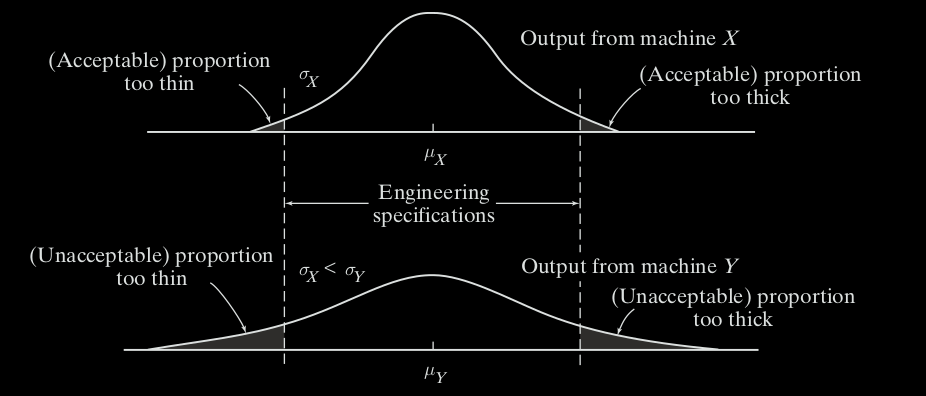
\includegraphics[scale=0.35]{Figure_9-3-1-neg.png}
	\vfill
\item[Mot. 2] To test $H_0:\mu_X=\mu_Y$ under the assumption $\sigma_X^2=\sigma_Y^2$, we need to first test $\sigma_X^2 = \sigma_Y^2$.
	\end{enumerate}
\end{frame}
%-------------- end slide -------------------------------%}}}
%-------------- start slide -------------------------------%{{{ 9.38
\begin{frame}
\centering
Testing $H_0:\sigma_X^2 = \sigma_Y^2$ \\[1em]
v.s.\\[1em]
(at the $\alpha$ level of significance)
\\
\vfill

\begin{minipage}{0.32\textwidth}
\centering
$H_1:\sigma_X^2 <\sigma_Y^2$:\\[1em]
Reject $H_0$ if \\[1em]
$s_Y^2/s_X^2\le F_{\alpha,m-1,n-1}$\\
\vspace{1.2em}
\phantom{aaa}
\end{minipage}
\begin{minipage}{0.32\textwidth}
\centering
$H_1:\sigma^2_X \ne \sigma^2_Y$:\\[1em]
Reject $H_0$ if \\[1em]
$s_Y^2/s_X^2 \ge F_{1-\alpha/2,m-1,n-1}$ or\\
$s_Y^2/s_X^2 \le F_{\alpha/2,m-1,n-1}$
\end{minipage}
\begin{minipage}{0.32\textwidth}
\centering
$H_1:\sigma^2_X>\sigma^2_Y$:\\[1em]
Reject $H_0$ if \\[1em]
$s_Y^2/s_X^2\ge F_{1-\alpha,m-1,n-1}$\\
\vspace{1.2em}
\phantom{aaa}
\end{minipage}
\end{frame}
%-------------- end slide -------------------------------%}}}
%-------------- start slide -------------------------------%{{{ 9.39
\begin{frame}
\begin{itemize}
	\item[E.g.] Electroencephalograms (EEG). \\[1em]
		Twenty inmates in a Canadian prison, randomly split into
		two groups of equal size: one in solitary confinement, one in their own cells.\\[1em]
		Measure the alpha waves.
		Whether the observed difference in variability is significant (set $\alpha=0.05$.)\\
		\vfill
		\begin{minipage}{0.45\textwidth}
			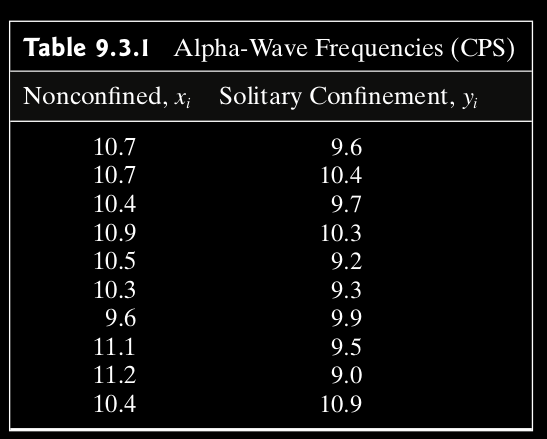
\includegraphics[scale=0.2]{Table_9-3-1-neg.png}
\end{minipage}
		\begin{minipage}{0.45\textwidth}
			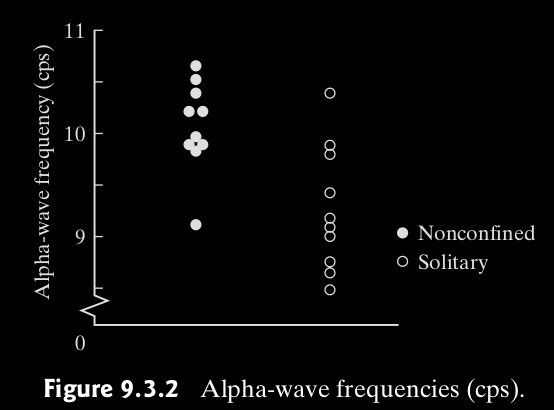
\includegraphics[scale=0.2]{Figure_9-3-2-neg.png}
\end{minipage}
\vfill
\item[Sol.] ... \myEnd
\end{itemize}
\end{frame}
%-------------- end slide -------------------------------%}}}
%-------------- start slide -------------------------------%{{{ 9.40
\begin{frame}
Another example here: \\[2em]
\url{https://www.itl.nist.gov/div898/handbook/eda/section3/eda359.htm}
\end{frame}
%-------------- end slide -------------------------------%}}}
